\documentclass[a4paper,12pt]{article}
\usepackage{graphicx}
\usepackage{fixltx2e}
\usepackage{amsmath}
\pagestyle{myheadings}
\graphicspath { {'/'} }
\begin{document}
	\author{Quang-Vinh DANG\\
COAST team - Inria Nancy}
	\title{Technical Report\\ Evaluation of Google Docs performance}\maketitle

\section{Introduction}

Google Docs can be considered as one of the most common collaborative editors nowadays. For the users that have experience with Microsoft Office, Google Docs is very easy to use and integrate.
Google claimed that Google Docs can support up to 50 users to modify a single document on the same time\footnote{ https://support.google.com/drive/answer/2494827?hl=en}, but there is no official definition so far for this situation.
We want to evaluate the performance of Google Docs in case of multiple concurrent users, not by using theoretic calculation, but by simulating real user behaviors on web browser, to see whether if Google Docs satisfy large scale setting of collaborative editing or not.

\section{Evaluation Method}
We evaluate the performance of Google Docs in term of delay, which defined as following:

\textit{We consider two users A and B who are modifying and viewing a same document on Google Docs by using web browser. User A performs a modification (such as insert character 'a') on his local document at the point of time t\textsubscript{1}. User B receives this modification (i.e, he can see the character 'a' appears on his local document) at the point of time t\textsubscript{2}. The delay is defined as $\Delta$t = t\textsubscript{2} - t\textsubscript{1}.}

To evaluate this delay, we setup the testing system as follows:
\begin{itemize}
	\item We use Selenium WebDriver Java 2.44.0\footnote{http://www.seleniumhq.org} to simulate user behavior.
	\item We configure a number of concurrent threads to simulate concurrent users.
	\begin{itemize}
		\item There is a special thread which act as reader: this thread does not modify the document but only read the document to record the modification it receives.
		\item There is another special thread which try to write special strings (the writer). These special strings will be read by the reader.
		\item There are another threads (dummy writers) which also write to the document, but their writings are only used to simulate concurrent users. Particularly, they will continuously write a non meaningful text.
		\item The actions of all threads are inserting and reading text, and there is no deletion.
	\end{itemize}
	\item The time when the writer insert a particular string and the time when the reader record this string on his document will be recorded and used to calculate the delay. To eliminate the difference in clock, both writer and reader are executed on a same computer.
\end{itemize}
We perform the evaluation with different settings:
\begin{itemize}
	\item We increase the number of user (the number of thread), from 1 (i.e, 1 writer and 1 reader), to 2 (i.e, 2 writers and 1 reader) up to 50 (50 writers and 1 reader).
	\item For each particular number of user, we change the typing speed of each user. The typing speed is defined as number of character each user type in one second. Our testing range is from 1 to 10. The regular typing speed is 2 characters per second\footnote{http://en.wikipedia.org/wiki/Typing}.
\end{itemize}

\section{Result}

The result of the evaluation is displayed in Fig. \ref{fig:google_docs1}. The y - axis shows the delay we observed in seconds, when the x - axis shows the settings of the evaluation. For instance, the x - label '10.01' means there are 10 writers and 1 reader in this evaluation, with the typing speed of each users are 1 character / second. 

For the number of user 40 and 50, we cannot increase the typing speed more than 1: Google Docs will immediately refused the connection.

\begin{figure}
		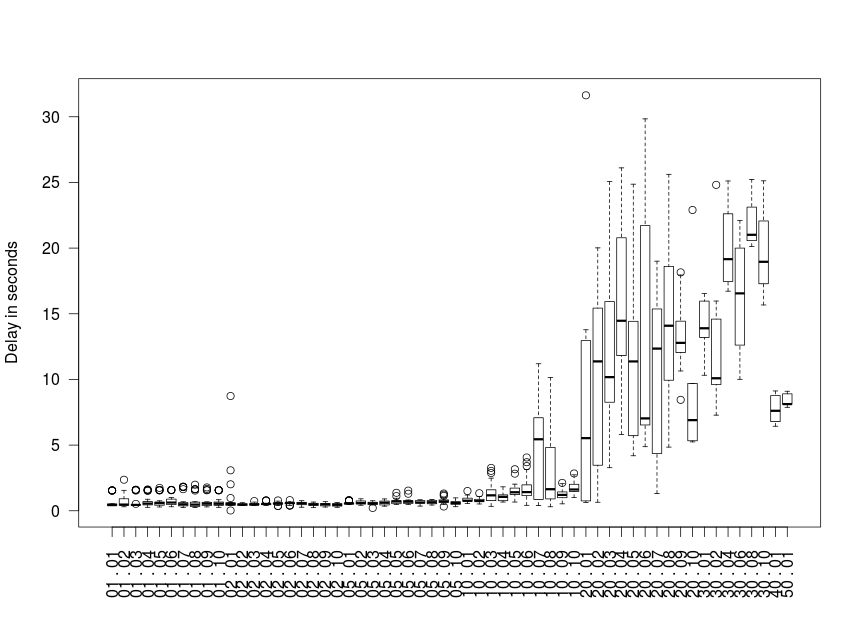
\includegraphics[width=\textwidth]{GoogleDocs}	
		\caption{Delays of Google Docs with different number of users and typing speed}
		\label{fig:google_docs1}
	\end{figure}
	
\section{Conclusion}
We measured the performance of Google Docs in real user behavior settings.

From the result, we can conclude: Google Docs works quite well with a small number of user (less than 10), but when the number of user increases, the delay increases so fast and it seems not appropriate to use in large scale settings.

On the other hand, the typing speed also affects to the performance. If users increase typing speed, more delay will be introduced.
	
\end{document}